%Fig Optical satellites:

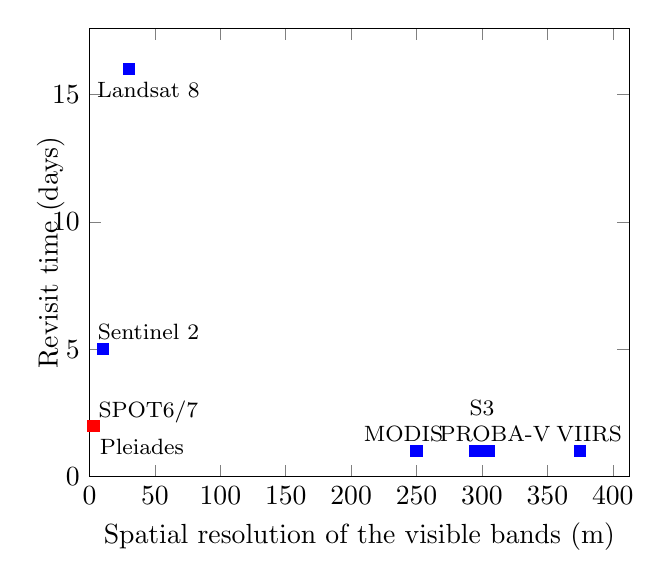
\begin{tikzpicture} 
	\begin{axis}[% 
		%coords={(xy): \thisrow{label}},%
		ylabel style={yshift=-0.4cm}, %shifting the y line text
	%	ylabel shift = 40 pt,
		ymin = 0,
		xmin=0, 
		xlabel={Spatial resolution of the visible bands (m)}, 
		ylabel={Revisit time (days)},
		xtick={0,50,100,150,200,250,300,350,400},
		ytick={0,5,10,15,20},
		scatter/classes={%
		b={mark=square*,blue},%
		r={mark=square*,red}}]
%	set(y, 'Units', 'Normalized', 'Position', [-2, 0.5, 2]);
		\addplot[scatter,only marks,%
		scatter src=explicit symbolic,
		point meta=explicit symbolic]%
		table[meta=label] {
    %    table[meta index=2]
			x y label 
			250 1 b  
			295 1 b
			305 1 b
			375 1 b
			3   2 r
			3   2 r
			30  16 b
			10  5 b
			};
	%	\node at (axis cs:0,0)

		\node [above] at (axis cs:  45,  14.5) {\footnotesize Landsat 8};
		\node [above] at (axis cs:  45,  1.7)  {\footnotesize SPOT6/7};
		\node [above] at (axis cs:  40,  0.5)  {\footnotesize Pleiades};
		\node [above] at (axis cs:  45,  5)    {\footnotesize Sentinel 2};
		\node [above] at (axis cs:  240,  1)   {\footnotesize MODIS};
		\node [above] at (axis cs:  300,  2)   {\footnotesize S3};
		\node [above] at (axis cs:  310,  1)   {\footnotesize PROBA-V};		
		\node [above] at (axis cs:  382,  1)   {\footnotesize VIIRS};
	\end{axis}
\end{tikzpicture}

%\begin{tikzpicture} 
%	\begin{axis}[% 
%	scatter/classes={% 
%		a={mark=square*,blue},% 
%		b={mark=square*,red},% 
%	}]
%%		xlabel={Spatial resolution of the visible bands (m)}, 
%%		ylabel={Revisit time (days)}]
%	\addplot[scatter,only marks,% 
%	scatter src=explicit symbolic]% 
%	table[meta=label] {
%	x y label
%	0.1 0.15 a 
%	0.85 0.52 b 
%	0.76 0.5 b 
%	0.55 0.32 c
%	}; 
%	\end{axis} 
%\end{tikzpicture}